\documentclass[10pt,twocolumn]{article}
\usepackage[T1]{fontenc}
\usepackage[utf8]{inputenc}
\usepackage{lmodern}
\usepackage[letterpaper,textwidth=7.16in,columnsep=0.16in,top=0.75in,bottom=1in]{geometry}
\usepackage{amsmath}
\usepackage{graphicx}
\usepackage{booktabs}
\usepackage{url}
\graphicspath{{figures/}}

\title{Deep-Learning Channel Estimation for Indoor\\Visible Light Communication with OFDM}
\author{Jaafar Salim\\University of Technology, Iraq}
\date{}

\begin{document}
\maketitle

\begin{abstract}
Visible light communication (VLC) reuses room lighting for data, and orthogonal frequency-division
multiplexing (OFDM) copes with the low-pass response of the light-emitting diode (LED). The receiver still
has to estimate the channel. We train a five-layer perceptron on 4,000 simulated channels of a
$5\times5\times3$~m room and compare it with least-squares (LS) and linear minimum mean-square error (MMSE)
estimation. At 20~dB the network lowers the estimation error by 10.4~dB with respect to LS, and its bit error
rate (BER) of $1.39\times10^{-4}$ equals that of a receiver with perfect channel knowledge.
\end{abstract}

\section{Introduction}
LED lighting can carry data at the same time as it lights a room~\cite{komine2004fundamental,elgala2011indoor}.
Because the LED acts as a low-pass filter, VLC systems commonly use OFDM, which turns the dispersive channel into
many flat subchannels~\cite{armstrong2009ofdm}. Pilot-based estimation of those subchannels is well understood
for radio links~\cite{coleri2002channel}, and neural estimators have been shown to help when the classic
assumptions do not hold~\cite{ye2018power,soltani2019deep}. This report measures how much a small network
helps in an indoor VLC link, and where the linear MMSE estimator fails.

\section{System Model}
The LED sits at the centre of the ceiling and the photodiode at desk height (Fig.~\ref{fig:room}). The
line-of-sight gain follows the Lambertian model~\cite{kahn1997wireless},
\begin{equation}
H_{\mathrm{LOS}} = \frac{(m+1)A}{2\pi d^2}\cos^m(\phi)\,T_s\,g(\psi)\cos(\psi),
\label{eq:los}
\end{equation}
where $m$ is the Lambertian order, $A$ the detector area and $d$ the distance. First reflections from the walls
and the 3~MHz bandwidth of the LED complete the frequency response. Each OFDM symbol has 64 subcarriers with a
pilot on every fourth one.

\begin{figure}[t]
\centering
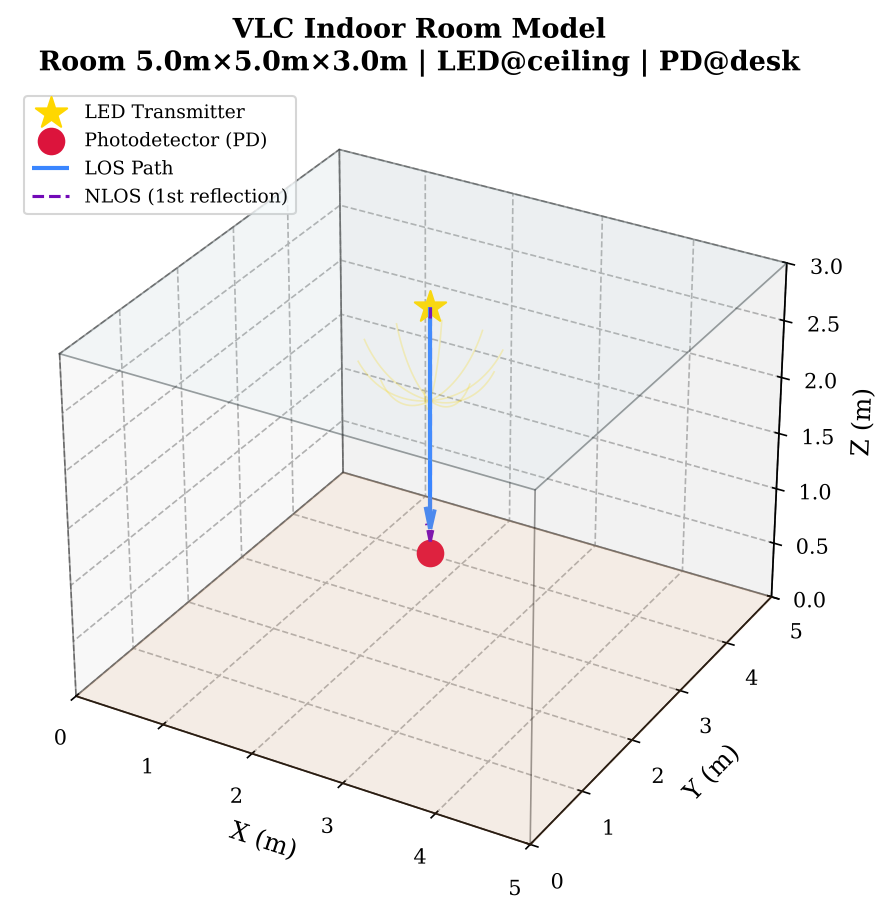
\includegraphics[width=0.8\columnwidth]{room}
\caption{Room geometry: LED on the ceiling, receiver plane at 0.85~m.}
\label{fig:room}
\end{figure}

\section{Estimators}
LS divides each received pilot by the transmitted one and interpolates between pilots. MMSE weights the LS
estimate with the channel correlation and a design signal-to-noise ratio (SNR), fixed here at 15~dB. The deep
learning (DL) estimator is a perceptron with layers of 512, 256, 256, 128 and 64 units, trained with
Adam~\cite{kingma2015adam} on channels from random positions and SNRs between 0 and 30~dB, as listed in
Table~\ref{tab:params}.

\begin{table}[t]
\centering
\caption{Simulation parameters}
\label{tab:params}
\begin{tabular}{@{}ll@{}}
\toprule
Room & $5\times5\times3$~m \\
LED semi-angle & $60^\circ$ \\
Subcarriers / pilots & 64 / 16 \\
Modulation & QPSK \\
Training set & 4,000 channels \\
\bottomrule
\end{tabular}
\end{table}

\section{Results}
Fig.~\ref{fig:mse} shows the estimation error. At 20~dB the DL estimate is 10.4~dB better than LS. The MMSE
estimator is better than LS near its design SNR, but above it the wrong noise assumption makes it worse than LS.

\begin{figure}[t]
\centering
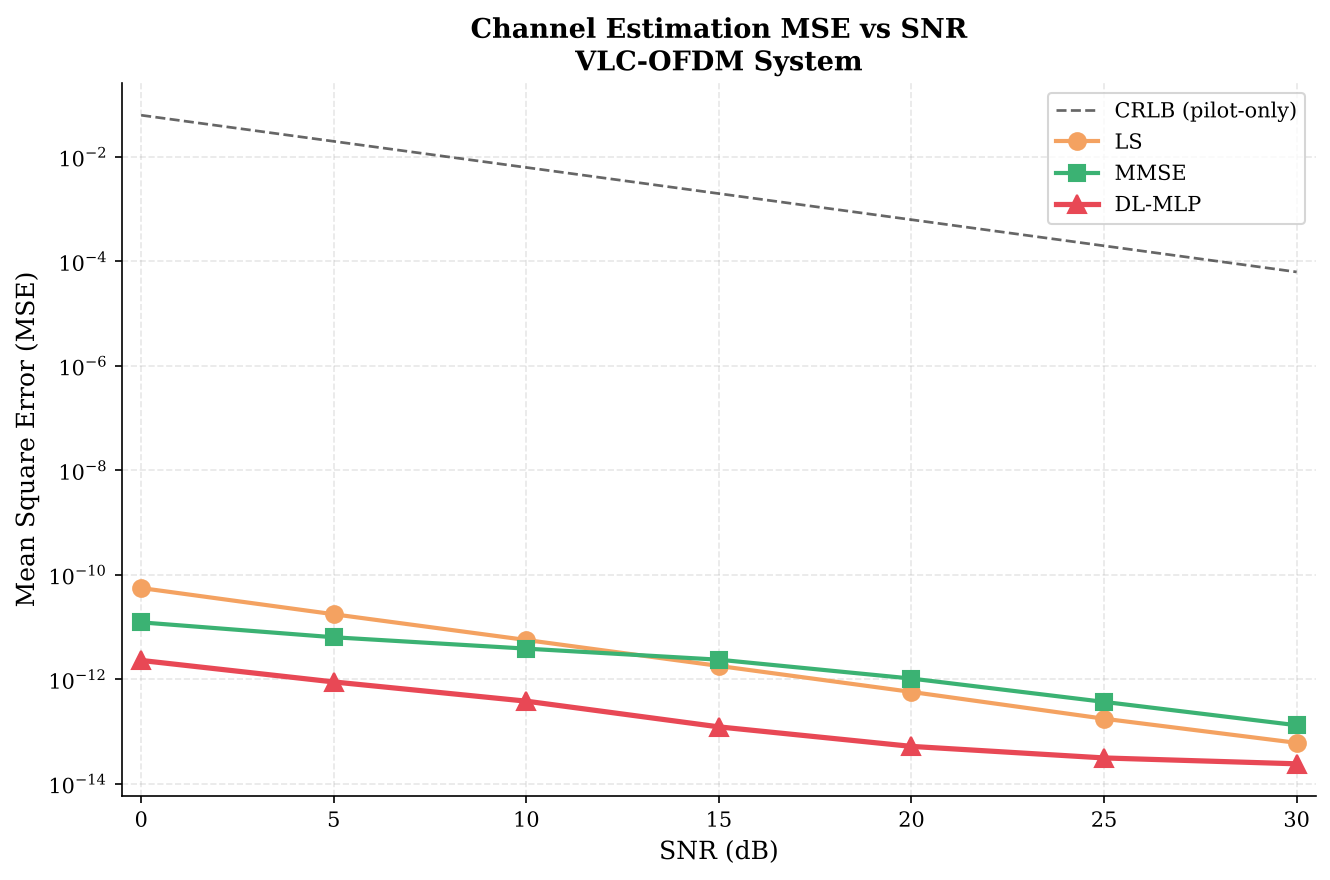
\includegraphics[width=\columnwidth]{mse_snr}
\caption{Mean-square error of the channel estimate against SNR.}
\label{fig:mse}
\end{figure}

The BER follows the same pattern (Fig.~\ref{fig:ber}). At 20~dB the DL receiver reaches $1.39\times10^{-4}$,
against $2.57\times10^{-3}$ for LS, which is 18 times fewer errors, and the same value as a receiver that knows
the channel exactly.

\begin{figure}[t]
\centering
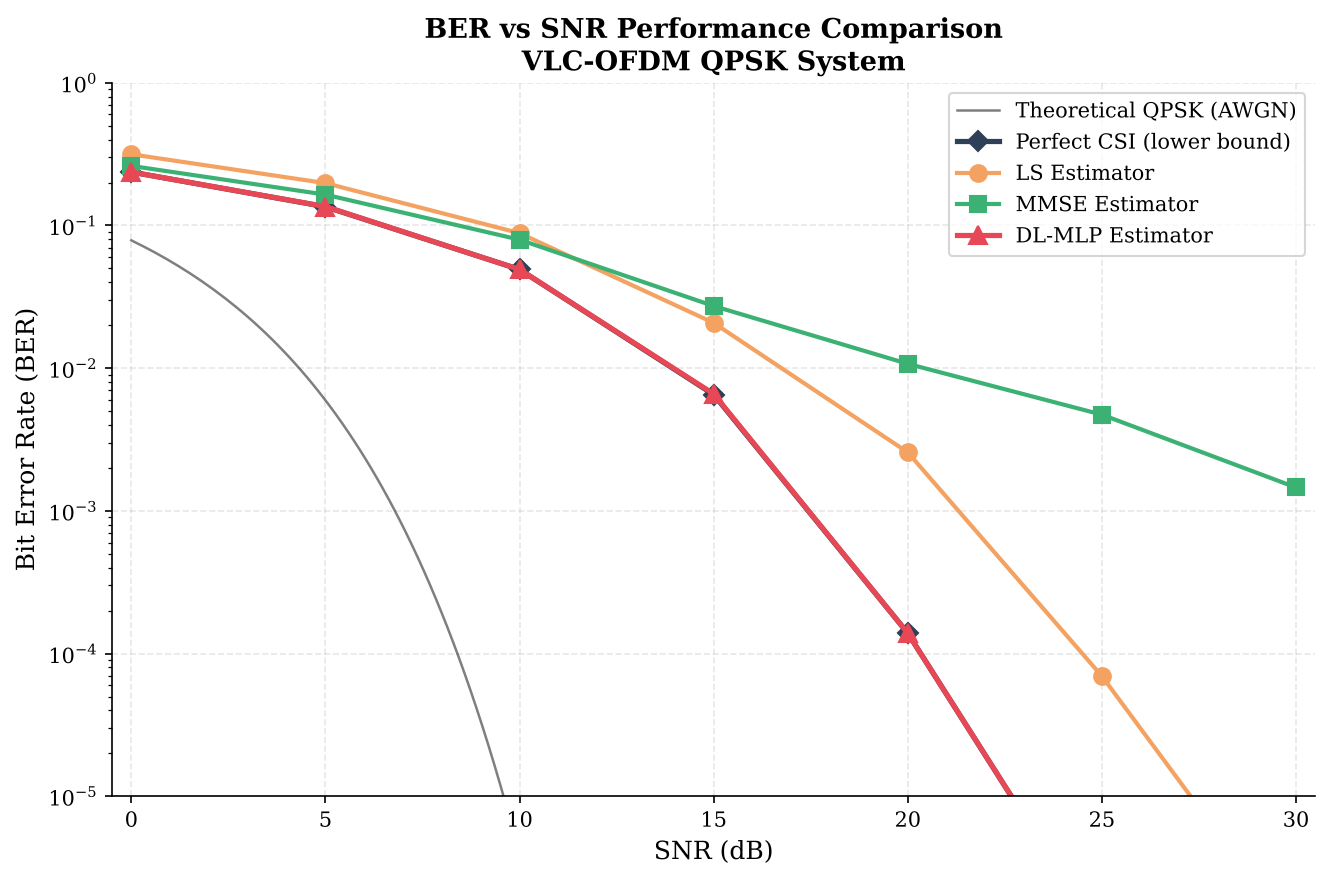
\includegraphics[width=\columnwidth]{ber_snr}
\caption{BER with QPSK for the three estimators and for perfect channel knowledge.}
\label{fig:ber}
\end{figure}

\section{Conclusion}
A small network trained across the full SNR range removes the estimation loss of an indoor VLC-OFDM link in
this simulation, while MMSE with a fixed design SNR degrades above it. The study is limited to one room, one
LED and simulated channels; a measured testbed is the next step.

\bibliographystyle{plain}
\bibliography{refs}
\end{document}
